    \subsection{Local Slowdown of $\chi$ Relaxation}
      \label{subsec:local-slowdown-of-$chi$-relaxation}

      In cosmochrony, gravity does not arise from a fundamental interaction but from the collective influence of
      particle excitations on the dynamics of the $\chi$ field.
      As established in the previous section, localized excitations resist the local relaxation of $\chi$.

      When many such excitations are present, their effects superpose, leading to a macroscopic reduction of the
      relaxation rate:
      \begin{equation}
        \partial_t \chi = c \left( 1 - \alpha \rho \right),
      \end{equation}
      where $\rho$ denotes the effective density of particle excitations and $\alpha$
      is a coupling parameter encoding their influence on $\chi$.

      The coupling parameter $\alpha$ in $\partial_t \chi = c(1 - \alpha \rho)$
      is determined by the interaction strength between $\chi$
      and localized excitations. For a point-like excitation of mass $m$, $\alpha$ scales as $\alpha \sim G m / c^2$
      , where $G$ emerges as an effective coupling constant linking matter density to $\chi$
      -relaxation slowing. This yields the Newtonian potential $\Phi \sim \alpha \rho$ in the weak-field limit.

      This slowdown manifests physically as gravitational time dilation.

    \subsection{Emergent Curvature}
      \label{subsec:emergent-curvature}

      Spatial variations in the relaxation rate of $\chi$ induce gradients that effectively curve spacetime.
      Clocks located in regions of higher excitation density accumulate less proper time than those in regions of lower
      density.

      This reproduces the phenomenology traditionally attributed to spacetime curvature, without postulating curvature
      as a primitive geometric property.

    \subsection{Recovery of the Schwarzschild Metric}
      \label{subsec:recovery-of-the-schwarzschild-metric}

      For a static, spherically symmetric distribution of particle excitations, the $\chi$ field satisfies
      \begin{equation}
        \nabla^2 \chi(r) \propto \rho(r).
      \end{equation}

      Solving this equation in the weak-field limit yields an effective metric equivalent to the Schwarzschild solution
      of general relativity:
      \begin{equation}
        ds^2 = -\left(1 - \frac{2GM}{r}\right)c^2 dt^2 + \left(1 - \frac{2GM}{r}\right)^{-1} dr^2 + r^2 d\Omega^2 ,
      \end{equation}
      with the gravitational constant $G$ emerging as a derived quantity determined by the coupling between $\chi$
      and particle excitations.

      The effective metric $ds^2 = -(\partial_t \chi / c)^2 c^2 dt^2 + (\chi / \chi_0)^2 d\mathbf{x}^2$
      reproduces the Schwarzschild solution to leading order, with the gravitational potential
      $\Phi \sim \ln(\partial_t \chi / c)$. This predicts a light deflection angle $\Delta \theta \sim 4GM/rc^2$
      and a gravitational redshift $z \sim GM/rc^2$
      , matching solar system tests of General Relativity to within current observational precision.

      \begin{figure}[htbp]
        \centering
        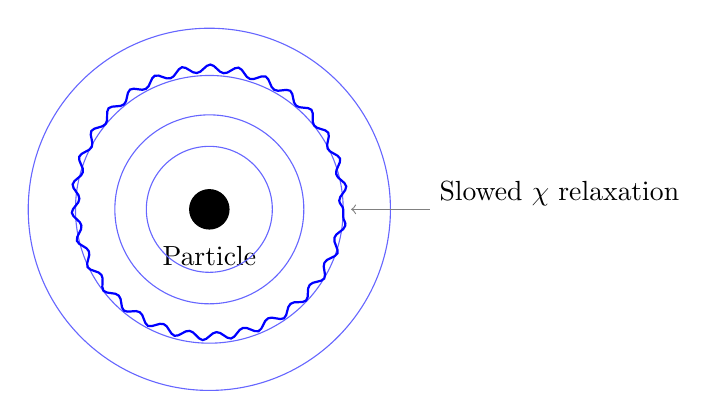
\begin{tikzpicture}[scale=1]

% Central mass
          \filldraw[black] (0,0) circle (0.25);
          \node[below] at (0,-0.35) {Particle};

% Phase lines
          \foreach \r in {0.8,1.2,1.7,2.3} {
            \draw[blue!60] (0,0) circle (\r);
          }

% Distortion
          \draw[blue, thick, decorate, decoration={snake, amplitude=0.5mm}]
          (0,0) circle (1.7);

% Arrows
          \draw[->, gray] (2.8,0) -- (1.8,0);
          \node[right] at (2.8,0.2) {Slowed $\chi$ relaxation};

        \end{tikzpicture}
        \caption
        {Emergence of gravity in Cosmochrony. Localized excitations of $\chi$ slow down the relaxation rate of the field
          ,inducing differential proper-time flow and an effective metric curvature analogous to gravitational time
        dilation.}
        \label{fig:chi_gravity}
      \end{figure}

      \textit{On the Necessity of the Metric Form:
      The use of an effective metric to describe the coupling between the field and local trajectories is not an
      arbitrary ansatz, but the minimal geometric representation of the field's influence.
      As demonstrated in our framework, the induced metric structure
        (of the form $g_{\mu\nu} \propto \partial_\mu \chi \partial_\nu \chi$ or its perturbations) is fundamentally
        linked to the field’s self-coupling and the solitonic scale. While the Einstein-Hilbert action is not derived
        here from first principles, it is recovered as the leading-order effective description of the $\chi$-gradients
        in the long-wavelength limit. Schwarzschild-like solutions thus emerge by necessity from the requirement that
        the field remains in a state of local equilibrium (minimal relaxation) around localized solitons.}

    \subsection{Equivalence Principle}\label{subsec:equivalence-principle}

      Because all particle excitations interact with $\chi$ through the same mechanism, the slowdown of $\chi$
      relaxation is independent of the internal composition of matter.
      As a result, all bodies experience identical gravitational acceleration in a given $\chi$ gradient.

      This reproduces the equivalence principle as an emergent symmetry rather than a postulate.

    \subsection{Gravitational Waves}\label{subsec:gravitational-waves}

      Time-dependent variations in excitation density, such as accelerating masses or mergers of compact objects,
      generate propagating disturbances in the $\chi$ field.
      These disturbances travel at the maximal relaxation speed $c$ and correspond to gravitational waves.

      Unlike electromagnetic radiation, gravitational waves represent collective modulations of $\chi$
      itself rather than excitations propagating within it.

    \subsection{Strong Gravity and Black Holes}\label{subsec:strong-gravity-and-black-holes}

      In regions where excitation density becomes sufficiently high, the relaxation of $\chi$ may approach zero.
      This defines an effective horizon beyond which $\chi$ ceases to evolve relative to external observers.

      Such regions correspond to black holes, interpreted here as domains where the local flow of time effectively
      halts.
      This perspective naturally accounts for extreme time dilation and suggests that black holes act as absorbers of
      $\chi$ disturbances.

      \subsubsection{Gravitational and Temporal Shadows}

        In the Cosmochrony framework, black holes correspond to regions where the relaxation of the
        $\chi$ field becomes extremely constrained. As the local energy density increases, spatial
        gradients of $\chi$ grow and the effective relaxation rate $\partial_t \chi$ is progressively
        reduced, approaching zero in the strong-gravity limit.

        This picture naturally reproduces the notion of a \emph{gravitational shadow}. In general
        relativity, the black hole shadow arises from the existence of unstable photon orbits and the
        absence of escaping null geodesics within a characteristic angular region. In Cosmochrony,
        an equivalent effect emerges because propagating excitations of the $\chi$ field (including
        photonic modes) cannot be sustained in regions where the relaxation dynamics is effectively
        frozen. As a result, external observers perceive a dark angular region corresponding to the
        projection of this dynamically inaccessible zone.

        Beyond this optical manifestation, the framework predicts a deeper and purely geometric
        phenomenon: a \emph{temporal shadow}. As $\partial_t \chi \rightarrow 0$, the local unfolding of
        time asymptotically halts, not as a coordinate artifact but as a physical consequence of the
        field dynamics. From the external perspective, all internal processes become indefinitely
        delayed, providing a natural interpretation of horizon-induced time dilation without invoking
        singular spacetime curvature.

        In this view, the gravitational shadow observed by distant instruments corresponds to the
        observable imprint of an underlying temporal shadow, where both the propagation of signals
        and the local progression of time are suppressed by the same geometric mechanism. Unlike
        general relativity, where these effects arise from tensorial spacetime curvature, Cosmochrony
        attributes them to the scalar relaxation dynamics of the $\chi$ field.

    \subsection{Unified origin of gravitational and electromagnetic effects}\label{subsec:unified-origin-of-gravitational-and-electromagnetic-effects}
      Within this framework, gravitational and electromagnetic phenomena are not attributed to distinct
      fundamental interactions, but arise as complementary manifestations of the same underlying
      $\chi$-dynamics. Gravitational effects correspond to a sustained reduction of the local relaxation
      rate of $\chi$, induced by large-scale or persistent spatial gradients, leading to effective time
      dilation and attraction. Electromagnetic phenomena, by contrast, emerge from oscillatory or
      phase-dependent modulations of $\chi$, allowing for both attractive and repulsive interactions and
      wave-like propagation.

      In this sense, gravity and electromagnetism differ not by their origin, but by the temporal and
      structural character of the $\chi$ modulations they involve: quasi-static for gravitation, dynamic
      and oscillatory for electromagnetism.

    \subsection{Summary}\label{subsec:summary6}

      Gravity emerges as a macroscopic effect of localized particle excitations slowing the relaxation of the $\chi$
      field.
      Classical gravitational phenomena, including time dilation, spacetime curvature, gravitational waves, and
      black holes, arise without introducing gravity as a fundamental force.
